\chapter{\MakeUppercase{Giới thiệu tổng quan}} 
\section{Bối cảnh và động lực phát triển}

\subsection{Xu hướng phát triển xe thông minh}

Trong kỷ nguyên chuyển đổi số và kết nối vạn vật (IoT), ngành công nghiệp ô tô toàn cầu đang trải qua một cuộc cách mạng mạnh mẽ từ các phương tiện cơ khí truyền thống sang xe thông minh (Smart Vehicles) và xe được định nghĩa bởi phần mềm (Software-Defined Vehicles - SDV). Theo báo cáo của McKinsey \& Company (2023)\cite{mckinsey2023}, thị trường xe thông minh toàn cầu dự kiến đạt 556 tỷ USD vào năm 2026 với tốc độ tăng trưởng hàng năm 12.5\%. Xu hướng này được thúc đẩy bởi ba yếu tố chính:

\begin{enumerate}
    \item Connectivity (Kết nối): Các phương tiện hiện đại được tích hợp khả năng kết nối Internet và giao tiếp V2X (Vehicle-to-Everything), cho phép trao đổi dữ liệu với hạ tầng giao thông, các phương tiện khác và điện thoại thông minh của người dùng.
    
    \item Electrification (Điện khí hóa): Sự bùng nổ của xe điện (EV) và xe Hybrid đòi hỏi các hệ thống điện tử phức tạp hơn để quản lý năng lượng, sạc pin và tối ưu hóa hiệu suất.
    
    \item Autonomous Driving (Tự lái): Các công nghệ ADAS (Advanced Driver Assistance Systems) và Autonomous Driving yêu cầu hàng trăm cảm biến, ECU và khả năng xử lý dữ liệu thời gian thực.
\end{enumerate}

\begin{figure}[htbp]
\centering
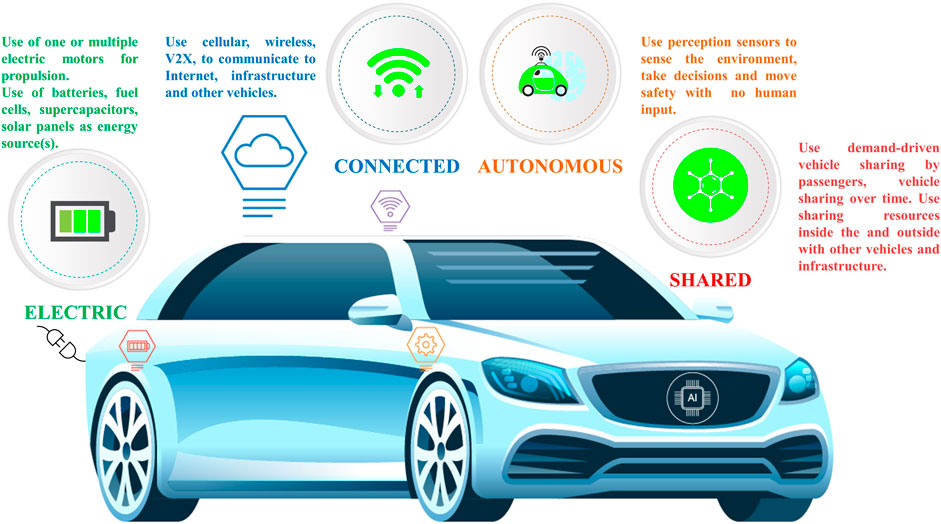
\includegraphics[width=0.8\textwidth]{image/section2/car.jpg}
\caption[Hệ sinh thái xe kết nối (Connected Vehicle Ecosystem)]{Hệ sinh thái xe kết nối (Connected Vehicle Ecosystem) (\textbf{Nguồn:} \href{https://www.frontiersin.org/journals/future-transportation/articles/10.3389/ffutr.2021.688482/full}{Frontiers})}
\label{fig:connected_vehicle}
\end{figure}

Trong bối cảnh này, hệ thống truy cập xe thông minh (Smart Car Access System) đã trở thành một trong những tính năng quan trọng nhất, không chỉ nâng cao trải nghiệm người dùng mà còn là nền tảng cho các dịch vụ Mobility-as-a-Service (MaaS) và Car Sharing trong tương lai. Xu hướng \textbf{"chìa khóa kỹ thuật số"} (Digital Key) đang dần thay thế các loại chìa khóa vật lý và Remote Keyless Entry (RKE) truyền thống, cho phép người dùng mở khóa, khởi động xe và cá nhân hóa cài đặt chỉ bằng điện thoại thông minh.

Các hãng ô tô hàng đầu như Tesla, BMW, Mercedes-Benz, và Hyundai đã triển khai các giải pháp Digital Key sử dụng công nghệ Bluetooth Low Energy (BLE), Near Field Communication (NFC) và Ultra-Wideband (UWB). Car Connectivity Consortium (CCC) - tổ chức gồm các thành viên như Apple, Samsung, Audi, BMW, General Motors - đã phát hành chuẩn Digital Key Release 3.0 vào năm 2021 \cite{ccc_digikey3}, sử dụng UWB để chống tấn công relay và đảm bảo secure ranging với độ chính xác centimet.

\begin{figure}[H]
\centering
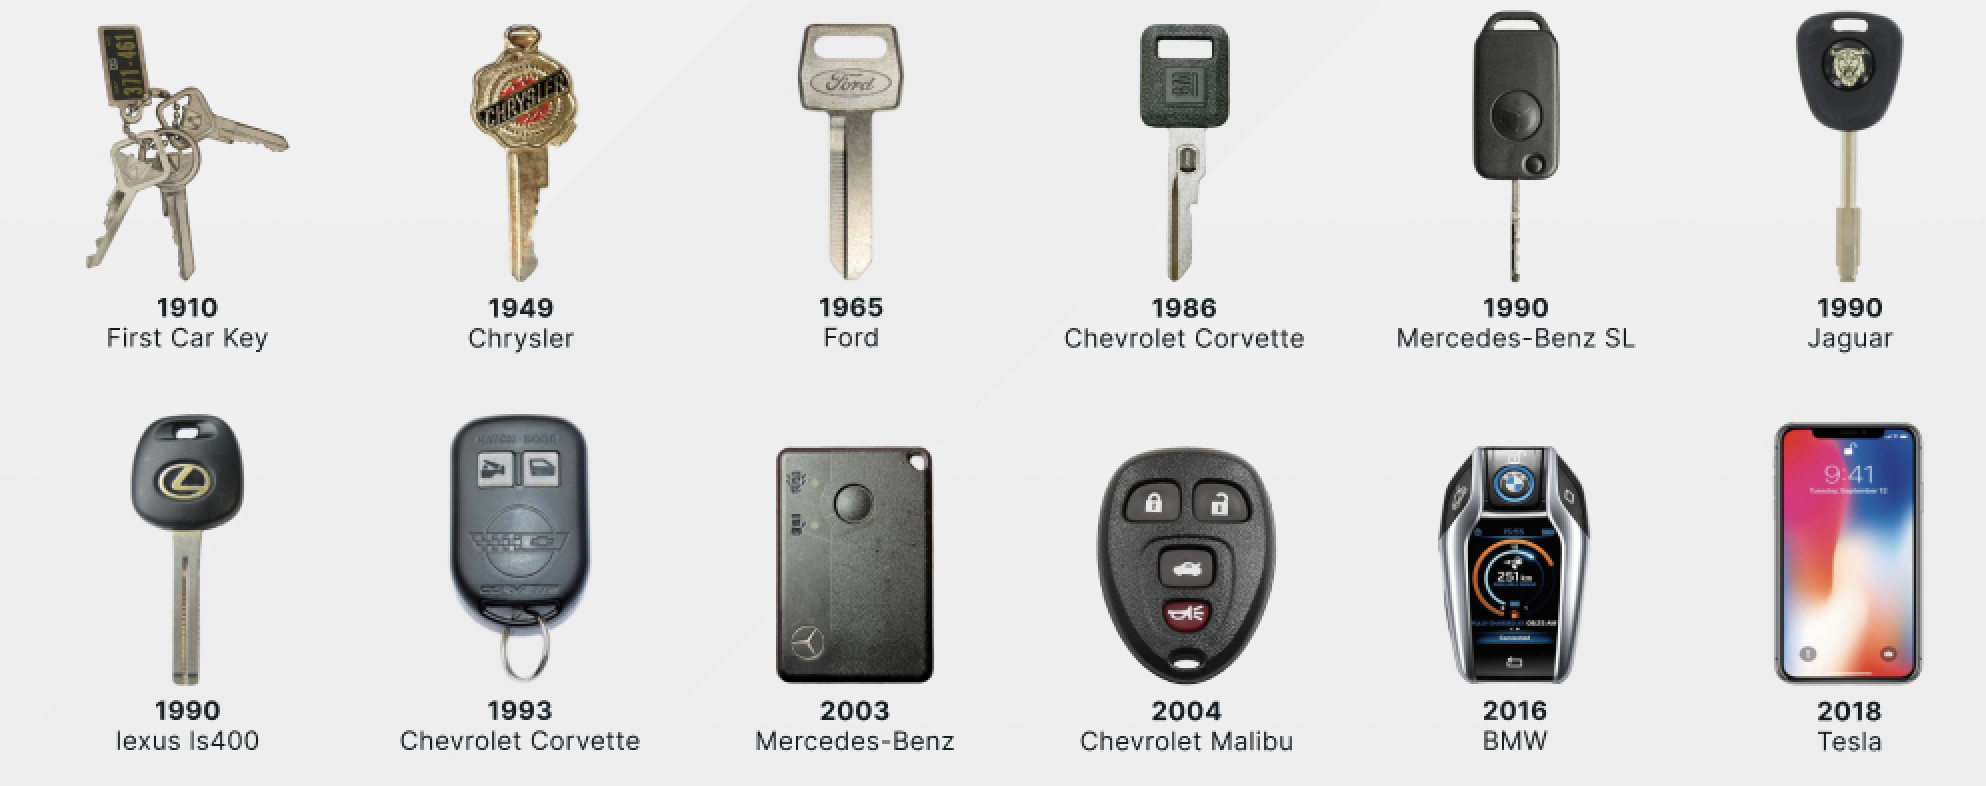
\includegraphics[width=0.8\textwidth]{image/section2/car3.png}
\caption{Công nghệ chìa khóa qua các thời kì}
\label{fig:digital_key_evolution}
\end{figure}

\subsection{Vấn đề bảo mật của các hệ thống Keyless Entry truyền thống}
Mặc dù công nghệ Keyless Entry mang lại sự tiện lợi vượt trội, các hệ thống truyền thống đang đối mặt với nhiều thách thức nghiêm trọng về bảo mật:
\begin{enumerate}
    \item \textbf{Tấn công chuyển tiếp (Relay Attack)} 
    
    Đây là mối đe dọa lớn nhất đối với hệ thống Passive Keyless Entry (PKE). Kẻ tấn công sử dụng hai thiết bị để khuếch đại và chuyển tiếp tín hiệu giữa chìa khóa (hoặc điện thoại) và xe, tạo ảo giác rằng chìa khóa đang ở gần xe. Nghiên cứu của Francillon et al. (2011) \cite{francillon2011relay} đã chứng minh hầu hết các xe sử dụng PKE đều dễ bị tấn công này, bao gồm cả các thương hiệu cao cấp như Audi A6, BMW X5, và Range Rover Sport.

    \begin{figure}[H]
    \centering
    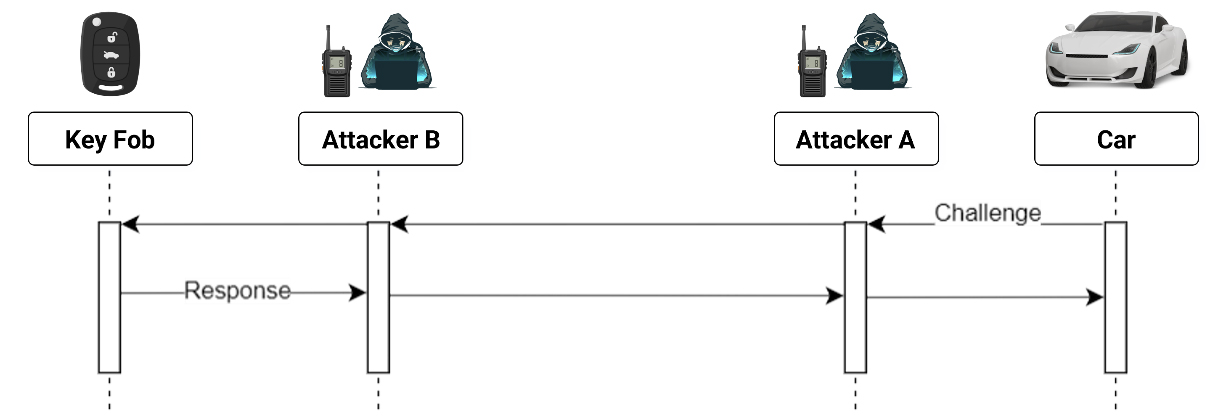
\includegraphics[width=0.85\textwidth]{image/section2/car2.jpg}
    \caption[Sơ đồ minh họa tấn công chuyển tiếp (Relay Attack) trên hệ thống Keyless Entry]{Sơ đồ minh họa tấn công chuyển tiếp (Relay Attack) trên hệ thống Keyless Entry (\textbf{Nguồn:} \href{https://www.automotiveworld.com/articles/mitigating-vulnerabilities-in-keyless-entry-systems/}{Automotive World})}
    \label{fig:relay_attack}
    \end{figure}

    Năm 2021, nhóm nghiên cứu của Lennert Wouters tại KU Leuven \cite{wouters2021tesla} đã công bố lỗ hổng bảo mật trên hệ thống BLE-only của Tesla Model 3 và Model Y, cho phép kẻ tấn công mở khóa và khởi động xe bằng cách relay các gói tin BLE. Tesla đã phải phát hành bản vá khẩn cấp để giảm thiểu rủi ro.
    
    \item \textbf{Tấn công phát lại (Replay Attack)} 
    
    Kẻ tấn công ghi lại tín hiệu mở khóa hợp lệ từ chìa khóa của người dùng và phát lại tín hiệu đó sau này để chiếm quyền kiểm soát. Mặc dù công nghệ mã hóa thay đổi (Rolling Code) đã được áp dụng, nhiều hệ thống vẫn tồn tại lỗ hổng do việc hiện thực hóa giao thức không đúng cách hoặc thiếu cơ chế xác thực thách thức - phản hồi (Challenge-Response) đủ mạnh.
    
    \item \textbf{Sao chép và giả mạo chìa khóa (Key Cloning \& Brute Force)} 
    
    Đối với các hệ thống có không gian khóa nhỏ hoặc không giới hạn tốc độ thử, kẻ tấn công có thể dò tìm mã khóa (Brute Force). Ngoài ra, sự phổ biến của các thiết bị phần cứng mã nguồn mở như Proxmark3 hay Flipper Zero cho phép sao chép dễ dàng các thẻ từ (RFID) hoặc Key Fob có độ bảo mật thấp.
    
    \item \textbf{Nghe lén dữ liệu (Eavesdropping)}
    
    Nếu giao thức truyền thông không đảm bảo tính bí mật chuyển tiếp (Forward Secrecy) và mã hóa mạnh, thông tin định danh nhạy cảm truyền qua sóng vô tuyến có thể bị kẻ gian thu thập và giải mã, tạo tiền đề cho các cuộc tấn công giả mạo về sau.
\end{enumerate}


\subsection{Các giải pháp Digital Key}

Để giải quyết các vấn đề bảo mật trên, các hãng ô tô đã phát triển nhiều giải pháp Digital Key khác nhau:
\begin{enumerate}
    \item \textbf{Tesla Model 3/Y}
    
    Tesla sử dụng kiến trúc đơn giản chỉ dựa trên BLE cho cả cấp phát khoá (Provisioning) và xác thực (Authentication). Ưu điểm của cách tiếp cận này là không cần phần cứng NFC, cho phép khoảng cách hoạt động xa (50--100\,m), và tích hợp sẵn với ứng dụng Tesla mobile app. Tuy nhiên, như đã đề cập, giải pháp này dễ bị tấn công chuyển tiếp (Relay Attack) do không có cơ chế xác minh khoảng cách vật lý. Chỉ số RSSI (Received Signal Strength Indicator) của BLE không đủ chính xác để phân biệt khoảng cách thực sự, với sai số có thể lên đến 10--15\%. \cite{wouters2021tesla,gomez2012overview,heydon2013bluetooth}

    \item \textbf{BMW Digital Key} 
    
    BMW là một trong những hãng đầu tiên triển khai Digital Key Release 3.0 của Car Connectivity Consortium \cite{ccc_digikey3}, sử dụng kết hợp cả ba công nghệ: NFC cho cấp phát khóa (chạm điện thoại vào B-pillar), BLE cho phát hiện thiết bị, và \textbf{UWB cho đo khoảng cách an toàn}. UWB có khả năng đo khoảng cách với độ chính xác $<10$\,cm và cơ chế đo thời gian bay (time-of-flight measurement) giúp chống lại tấn công relay một cách hiệu quả \cite{ieee802154z,sidorenko2020accurate}. Tuy nhiên, giải pháp này yêu cầu phần cứng đắt tiền (chip UWB khoảng \$50), chỉ hỗ trợ một số mẫu iPhone mới nhất (iPhone~11 trở lên), và sử dụng giao thức độc quyền của BMW.

    \item \textbf{NXP CarKey Solution} 
    
    NXP Semiconductors cung cấp giải pháp CarKey dựa trên NFC Forum Type~4 Tag và Secure Element (SE) để lưu trữ khóa số \cite{iso14443,iso7816}. Ưu điểm của giải pháp này là mức độ bảo mật phần cứng cao (chip SE có khả năng chống can thiệp vật lý), tuân thủ tiêu chuẩn Global Platform, và hỗ trợ nhiều điện thoại cùng lúc. Nhược điểm là chi phí cao do cần chip SE (khoảng \$5--10 cho mỗi đơn vị), luồng cấp phát khóa phức tạp, và phụ thuộc nhà cung cấp (Vendor lock-in) vào hệ sinh thái của NXP.

\end{enumerate}


Từ phân tích các giải pháp hiện có, có thể thấy tồn tại một trade-off giữa bảo mật, chi phí và tính khả thi triển khai:

\begin{itemize}
    \item Các giải pháp BLE (Tesla) có chi phí thấp nhưng bảo mật chưa tối ưu
    \item Các giải pháp NFC + UWB (BMW) có bảo mật cao nhưng yêu cầu phần cứng đắt đỏ và hỗ trợ thiết bị hạn chế
    \item Các giải pháp dựa trên SE (NXP) có bảo mật phần cứng tốt nhưng chi phí cao và phức tạp
\end{itemize}

\begin{figure}[H]
\centering
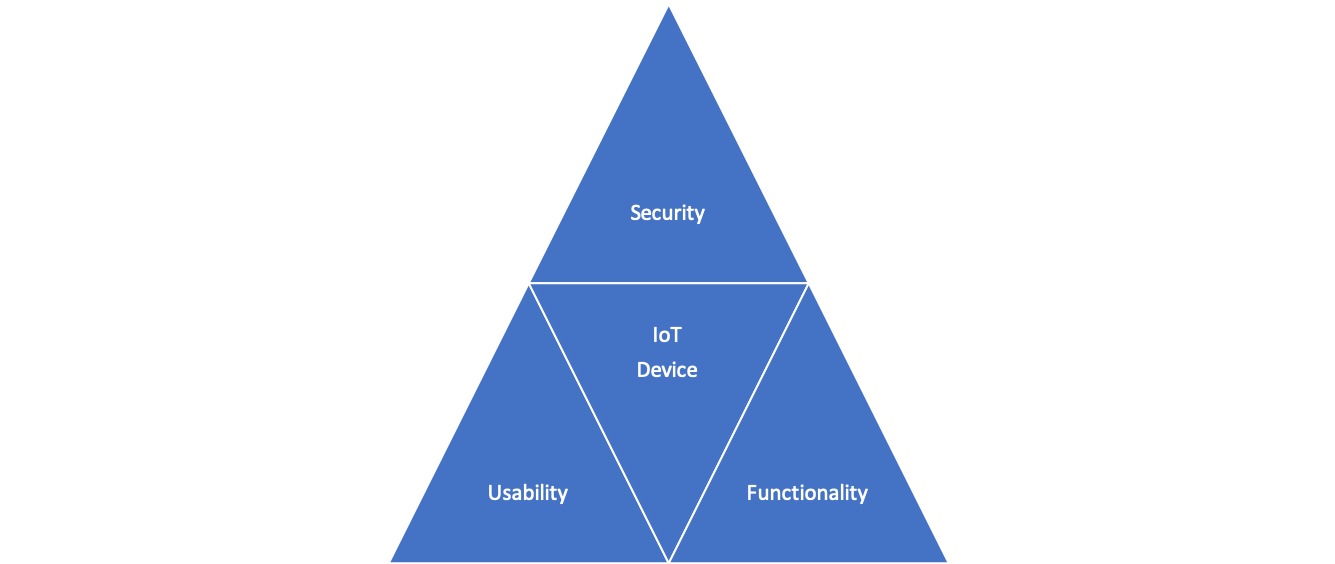
\includegraphics[width=0.75\textwidth]{image/section2/car4.png}
\caption[Trade-off giữa bảo mật, chi phí và tính khả thi của các giải pháp Digital Key]{Trade-off giữa bảo mật, chi phí và tính khả thi của các giải pháp Digital Key}
\label{fig:tradeoff}
\end{figure}

Đối với thị trường Việt Nam và các nước đang phát triển, nhu cầu về một giải pháp cân bằng giữa bảo mật và chi phí là rất cấp thiết. Các yêu cầu cụ thể bao gồm:

\begin{enumerate}
    \item \textbf{Bảo mật cao:} Tuân thủ các chuẩn mật mã quốc tế (NIST) \cite{nist_ecdh, fips186}, chống được Replay Attack và MITM Attack. Giảm thiểu Relay Attack mức độ tối đa có thể với công nghệ NFC + BLE và UWB trong tương lai.
    
    \item \textbf{Chi phí hợp lý:} Giải pháp sử dụng phần cứng sẵn có, các mã nguồn mở (open-source software stack), và không yêu cầu các chip chuyên dụng (SE, UWB) trong giai đoạn thử nghiệm.

    \item \textbf{Dễ triển khai:} Quy trình cấp phát khoá ban đầu đơn giản (NFC tap), hỗ trợ đa nền tảng (iOS và Android), và có khả năng tích hợp với các hệ thống ECU ô tô trong tương lai.

    \item \textbf{Khả năng nghiên cứu:} Mã nguồn mở, tài liệu hỗ trợ đầy đủ, có thể dùng làm tài liệu học tập cho sinh viên và kỹ sư trong nước.
\end{enumerate}

\section{Bối cảnh thị trường ô tô Việt Nam}

Tại Việt Nam, thị trường ô tô đang có tốc độ tăng trưởng ấn tượng với doanh số xe du lịch đạt hơn 300,000 chiếc trong năm 2023 (theo VAMA \cite{vama2023}). Người tiêu dùng ngày càng khắt khe về các tính năng công nghệ và tiện nghi, đặc biệt là thế hệ trẻ quen với smartphone và các thiết bị IoT. Chính phủ cũng đang đẩy mạnh đầu tư vào nghiên cứu và phát triển công nghiệp ô tô nội địa, với mục tiêu giảm phụ thuộc vào công nghệ nhập khẩu và tham gia sâu hơn vào chuỗi giá trị toàn cầu.

\begin{figure}[H]
\centering
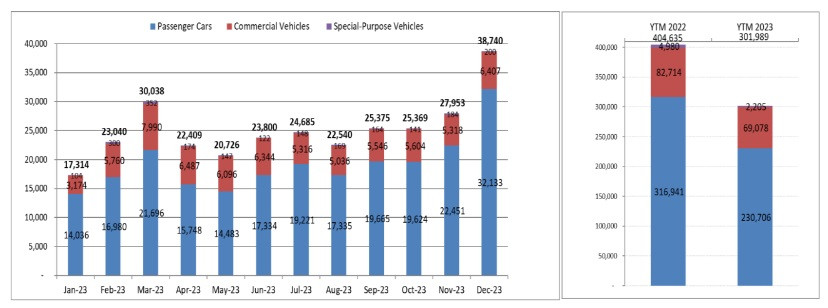
\includegraphics[width=0.8\textwidth]{image/section2/car5.jpg}
\caption[Tăng trưởng thị trường ô tô Việt Nam (Nguồn: VAMA 2023)]{Tăng trưởng thị trường ô tô Việt Nam (Nguồn: VAMA 2023) \cite{vama2023}}
\label{fig:vietnam_market}
\end{figure}

Việc nghiên cứu các giải pháp Smart Car Access trên nền tảng vi điều khiển và mô phỏng ECU không chỉ phù hợp với định hướng phát triển công nghệ quốc gia mà còn là bước đệm quan trọng để:

\begin{itemize}
    \item Kỹ sư Việt Nam tiếp cận và làm chủ các công nghệ lõi trong Automotive Security
    \item Xây dựng năng lực R\&D cho các doanh nghiệp Tier-2, Tier-3 trong chuỗi cung ứng ô tô
    \item Cung cấp giải pháp Aftermarket cho các xe đã qua sử dụng tại thị trường nội địa
    \item Tạo nền tảng cho các Startup công nghệ ô tô và IoT trong nước
\end{itemize}

Đề tài này hướng đến việc phát triển một \textit{\textbf{tài liệu tham khảo}} mã nguồn mở cho hệ thống truy cập xe thông minh (Smart Car Access) sử dụng kiến trúc kết hợp NFC--BLE, với khả năng chuyển đổi sang các ECU ô tô và mở rộng tích hợp UWB. Giải pháp được xây dựng dựa trên các chuẩn quốc tế (NIST, ISO) \cite{nist_ecdh, iso14443}, đồng thời tối ưu hoá cho chi phí nghiên cứu và triển khai tại các thị trường đang phát triển.

\section{Yêu cầu và mục tiêu đề tài}

\subsection{Yêu cầu đề tài}

Đề tài tập trung vào việc nghiên cứu và triển khai một hệ thống truy cập xe thông minh (Smart Car Access) sử dụng công nghệ truyền thông không dây hiện đại trên nền tự vi điều khiển. Hệ thống có chức năng chính là xác thực người dùng, thiết lập kết nối an toàn và điều khiển truy cập xe tự động, định hướng tuân thủ theo các tiêu chuẩn công nghiệp hiện hành. Đề tài yêu cầu đảm bảo các tiêu chí sau:

\begin{enumerate}
    \item \textbf{Tích hợp công nghệ truyền thông không dây:}
    
    Hệ thống phần cứng phải tích hợp thành công và đồng bộ các module giao tiếp \textbf{NFC (Near Field Communication)}, \textbf{BLE (Bluetooth Low Energy)} và \textbf{UWB (Ultra-Wideband)}. NFC đảm nhiệm vai trò đăng ký thiết bị ban đầu (Provisioning) với yêu cầu về tiếp xúc vật lý ở khoảng cách gần, nhằm đảm bảo tính bảo mật cốt lõi trong giai đoạn thiết lập. BLE thực hiện quá trình thiết lập kênh liên lạc an toàn và xác thực (Authentication) với phạm vi hoạt động rộng hơn. Đặc biệt, công nghệ UWB đã được hiện thực hóa để đóng vai trò then chốt trong việc đo lường và xác minh khoảng cách an toàn (Secure Distance Verification), giúp ngăn chặn triệt để các rủi ro giả mạo vị trí.

    \item \textbf{Phát triển ứng dụng Smart Car:}
    
    Xây dựng ứng dụng di động đa nền tảng (Cross-platform) đóng vai trò như một ``chìa khóa kỹ thuật số'' (Digital Key). Ứng dụng cần có khả năng giao tiếp liên tục với bộ điều khiển phương tiện thông qua nền tảng NFC/BLE/UWB, đồng thời hiển thị trạng thái kết nối và trạng thái xe (locked/unlocked). Hệ thống hỗ trợ quản lý xác thực người dùng thông qua Firebase và lưu trữ các khóa mật mã (Cryptographic Keys) một cách an toàn trên thiết bị.

    \item \textbf{Xây dựng giao thức bảo mật:}
    
    Hệ thống cần triển khai các giao thức mật mã tuân thủ các chuẩn quốc tế (NIST) \cite{nist_ecdh, fips186} nhằm đảm bảo mức độ bảo mật cao. Giải pháp sử dụng Elliptic Curve Cryptography (ECC) cho quá trình trao đổi khóa (Key Exchange) và chữ ký số (Digital Signature), kết hợp với mã hóa đối xứng (Symmetric encryption) cho truyền tải dữ liệu. Cơ chế xác thực hai chiều (Mutual authentication) được duy trì để chống lại các tấn công trung gian (Man-in-the-Middle -- MITM attack). Để củng cố toàn diện, giao thức bảo mật thiết lập sự ràng buộc mật mã chặt chẽ giữa phiên kết nối BLE và luồng dữ liệu đo khoảng cách của UWB, kết hợp cơ chế chống Replay Attack thông qua việc sử dụng khóa tạm thời (ephemeral keys) và giới hạn thời gian phiên làm việc.

    \item \textbf{Mô phỏng hệ thống điều khiển xe:}
    
    Thiết kế và lập trình bộ điều khiển phương tiện trên vi điều khiển ESP32-S3, đóng vai trò mô phỏng bộ điều khiển điện tử (ECU) trong giai đoạn nghiên cứu. Hệ thống này sẽ tiếp nhận tín hiệu đã được xác thực từ ứng dụng di động, kết hợp với dữ liệu định vị để đưa ra quyết định điều khiển chính xác. Kiến trúc phần mềm được thiết kế theo mô hình phân lớp (Layered architecture) giúp thuận tiện cho việc chuyển đổi sang các hệ thống ECU ô tô thực tế trong tương lai.
\end{enumerate}

\subsection{Mục tiêu đề tài}

Mục tiêu cốt lõi của đề tài là xây dựng một kiến trúc hệ thống truy cập xe an toàn theo chuẩn CCC \cite{ccc_digikey3}, đáng tin cậy và có tính mở rộng cao, làm nền tảng cho việc nghiên cứu và phát triển các giải pháp automotive security tại Việt Nam. Cụ thể bao gồm:

\begin{enumerate}
    \item \textbf{Nghiên cứu và triển khai kiến trúc kết hợp NFC-BLE-UWB:}
    
    Thiết kế và tích hợp hệ thống giao tiếp đa không gian: NFC cho quá trình nạp khóa (Provisioning), BLE cho quá trình xác thực dữ liệu và UWB cho định vị không gian chính xác. Phân tích ưu nhược điểm của từng công nghệ và đề xuất phương án phối hợp tối ưu nhằm cân bằng giữa tính bảo mật, sự tiện dụng và chi phí triển khai.
    
    \item \textbf{Phát triển giao thức xác thực và định vị an toàn:}
    
    Đề xuất và triển khai giao thức xác thực nhiều giai đoạn dựa trên các tiêu chuẩn mật mã NIST \cite{nist_ecdh, fips186}. Phân tích các hình thức tấn công phổ biến như tấn công tiếp sóng (Relay attack), tấn công phát lại (Replay attack), tấn công xen giữa (MITM) và nghe lén (Eavesdropping). Chứng minh tính đúng đắn của giao thức thông qua phân tích bảo mật, kết hợp xác minh khoảng cách vật lý thực tế để loại bỏ hoàn toàn các vector tấn công từ xa.
    
    \item \textbf{Thiết kế kiến trúc phần mềm với mô hình FSM:}
    
    Xây dựng máy trạng thái hữu hạn (Finite State Machine - FSM) để quản lý toàn bộ vòng đời hoạt động từ nạp khóa, xác thực định danh đến đo lường khoảng cách và mở khóa xe. Áp dụng các mẫu thiết kế (Design patterns) và thực hành tốt nhất trong lập trình hệ thống nhúng để đảm bảo mã nguồn dễ bảo trì, dễ kiểm thử và có khả năng mở rộng.
    
    \item \textbf{Đánh giá hiệu năng và bảo mật:}
    
    Thực hiện kiểm thử toàn diện bao gồm: đánh giá hiệu năng giao tiếp, độ chính xác của đo lường khoảng cách UWB, kiểm thử độ tin cậy (tỷ lệ thành công, phân tích lỗi) và đánh giá an ninh (kiểm chứng khả năng ngăn chặn tấn công). Tham khảo các giải pháp thương mại (như của Tesla, BMW) để đánh giá tính cạnh tranh của đề tài. Xác định các hạn chế còn tồn tại và đề xuất lộ trình phát triển tiếp theo.
    
    \item \textbf{Xây dựng tài liệu tham chiếu mã nguồn mở:}
    
    Phát triển một tài liệu tham chiếu (Reference implementation) hoàn chỉnh kèm theo hướng dẫn chi tiết, chú thích mã nguồn và báo cáo kỹ thuật để phục vụ mục đích học tập và nghiên cứu.
\end{enumerate}

\section{Cấu trúc báo cáo Đồ án}
Báo cáo đồ án tốt nghiệp được tổ chức thành năm chương với nội dung như sau:

\begin{itemize}
    \item \textbf{Chương 1 - Giới thiệu:}\\
    Trình bày bối cảnh phát triển của công nghệ xe thông minh và xu hướng chìa khóa kỹ thuật số (Digital Key), đồng thời phân tích các vấn đề bảo mật của hệ thống mở khóa không chìa truyền thống (Keyless Entry), đặc biệt là lỗ hổng Relay Attack. Nội dung chương tập trung làm rõ động lực thực hiện đề tài là xây dựng một hệ thống tuân thủ tiêu chuẩn công nghiệp CCC (Car Connectivity Consortium) Release 3 \cite{ccc_digikey3}, các yêu cầu kỹ thuật cần đạt được, mục tiêu nghiên cứu cụ thể, và những đóng góp chính của đề tài đối với lĩnh vực an ninh ô tô (Automotive security) và hệ thống kết nối vạn vật (Embedded IoT).

    \item \textbf{Chương 2 - Cơ sở lý thuyết:}\\
    Trình bày các nền tảng lý thuyết liên quan đến giao tiếp không dây, bao gồm giao tiếp tầm ngắn NFC (Near Field Communication), BLE (Bluetooth Low Energy), và đi sâu vào công nghệ băng tần siêu rộng UWB (Ultra-Wideband) với cơ chế đo khoảng cách an toàn (Secure Ranging / Time of Flight). Bổ sung các khái niệm cốt lõi về \textbf{kiến trúc chuẩn CCC} \cite{ccc_digikey3}. Bên cạnh đó, chương cung cấp kiến thức nền tảng về mật mã học hiện đại (ECC, trao đổi khóa ECDH, mã hóa đối xứng AES-GCM) và lý thuyết về Điện toán đám mây (Cloud Computing) ứng dụng trong việc lưu vết (logging) và phát hiện bất thường.

    \item \textbf{Chương 3 - Phân tích và thiết kế hệ thống:}\\
    Chương này trình bày quá trình phân tích yêu cầu hệ thống chức năng và phi chức năng. Kiến trúc tổng thể được \textbf{tái thiết kế bám sát chuẩn CCC} \cite{ccc_digikey3}, bao gồm ba thành phần chính: bộ điều khiển phương tiện (Vehicle Edge), ứng dụng di động (Mobile Client) và \textbf{hệ thống đám mây (Cloud Backend)}. Chương mô tả chi tiết thiết kế giao thức bảo mật đa lớp gồm: Giao dịch tiêu chuẩn (Standard Authentication) để cấp khóa an toàn lần đầu, Giao dịch nhanh (Fast Authentication) tối ưu cho việc tự động mở cửa (Auto BLE) hàng ngày, và đặc biệt là Phiên UWB (UWB Session) để xác thực khoảng cách vật lý. Đồng thời, trình bày thiết kế luồng gửi dữ liệu log thời gian thực lên Cloud phục vụ cảnh báo bảo mật.

    \item \textbf{Chương 4 - Triển khai hệ thống:}\\
    Chương này trình bày quá trình hiện thực hóa hệ thống trên phần cứng nhúng, ứng dụng di động và đám mây. Nội dung tập trung mô tả việc lập trình cho vi điều khiển ESP32-S3 kết hợp \textbf{module UWB}, tổ chức cấu trúc dữ liệu theo chuẩn CCC, và tích hợp các thư viện mật mã. Đồng thời, trình bày việc xây dựng ứng dụng di động Flutter đa nền tảng và triển khai kênh kết nối 4G/WiFi đẩy dữ liệu log đóng/mở cửa lên dịch vụ Firebase, làm cơ sở để phát hiện các truy cập bất thường và gửi thông báo (Push Notification) đến người dùng.

    \item \textbf{Chương 5 - Kết quả và đánh giá:}\\
    Chương này trình bày các kết quả đạt được từ việc triển khai và thử nghiệm hệ thống trong điều kiện thực tế. Tiến hành đo đạc, so sánh độ trễ giữa Standard và Fast Authentication, đánh giá độ chính xác của khoảng cách UWB, cũng như tốc độ cảnh báo từ Cloud.

    \item \textbf{Chương 6 - Kết luận và định hướng phát triển:}\\
    Chương này tổng kết các kết quả chính của đồ án, khái quát giá trị khoa học và thực tiễn đạt được, đồng thời nêu rõ các hạn chế còn tồn tại và định hướng mở rộng trong tương lai.
\end{itemize}